\chapter{Технологический раздел}
\label{cha:impl}

В данном разделе будут составлены требования к программному обеспечению, выбраны средства реализации и определены тестовые данные.

\section{Требования к программному обеспечению}
Требования к вводу:
\begin{itemize}
    \item $n_1, m_1 \in \mathbb{N}$ - размеры первой матрицы;
    \item $n_2, m_2 \in \mathbb{N}$ - размеры второй матрицы;
    \item $n1 \cdot{} m1$ действительных чисел, разделенных символами-разделителями (пробел, перенос строки, табуляция и т.п.) - элементы первой матрицы, перечисленные построчно;
    \item $n2 \cdot{} m2$ действительных чисел, разделенных символами-разделителями - элементы второй матрицы, перечисленные построчно.
\end{itemize}
Требования к выводу:
\begin{itemize}
    \item результат умножения матриц.
\end{itemize}
Требования к программе:
\begin{itemize}
    \item выбор алгоритма происходит через аргументы командной строки путём передачи его номера:
        \begin{enumerate}[1)]
            \item стандартный алгоритм;
            \item алгоритм Винограда;
            \item модифицированный алгоритм Винограда.
        \end{enumerate}
\end{itemize}

\section{Средства реализации}
Для реализации программы вычисления редакционного расстояния мной был выбран язык программирования C++. В рамках текущей задачи данный язык программирования имеет ряд существенных преимуществ:
\begin{itemize}
    \item Статическая типизация;
    \item Близость к низкоуровневому C при наличии многих возможностей высокоуровненных языков;
    \item Встроенная библиотека std::chrono, позволяющая измерять процессорное время \cite{chronoart}.
\end{itemize}

\section{Листинги кода}

\noindent\begin{minipage}{\textwidth}
\begin{lstlisting}[caption=Классический алгоритм]
void ClassicMul(double **res, double **matrix1, double **matrix2,
                size_t n, size_t m, size_t r)
{
    for (size_t i = 0; i < n; i++)
    {
        for (size_t j = 0; j < m; j++)
        {
            res[i][j] = 0;

            for (size_t k = 0; k < r; k++)
            {
                res[i][j] += matrix1[i][k] * matrix2[k][j];
            }
        }
    }
}
\end{lstlisting}
\end{minipage}

\begin{lstlisting}[caption=Алгоритм Винограда]
void WinogradMul(double **res, double **matrix1, double **matrix2,
                 size_t n, size_t m, size_t r)
{
    double *mulh = new double[n]();
    double *mulv = new double[m]();

    for (size_t i = 0; i < n; i++)
    {
        for (size_t j = 0; j < r / 2; j++)
        {
            mulh[i] = mulh[i] + matrix1[i][2 * j] * matrix1[i][2 * j + 1];
        }
    }

    for (size_t j = 0; j < m; j++)
    {
        for (size_t i = 0; i < r / 2; i++)
        {
            mulv[j] = mulv[j] + matrix2[2 * i][j] * matrix2[2 * i + 1][j];
        }
    }

    for (size_t i = 0; i < n; i++)
    {
        for (size_t j = 0; j < m; j++)
        {
            res[i][j] = -(mulh[i] + mulv[j]);

            for (size_t k = 0; k < r / 2; k++)
            {
                res[i][j] = res[i][j] +
                            (matrix1[i][2 * k] + matrix2[2 * k + 1][j]) *
                            (matrix1[i][2 * k + 1] + matrix2[2 * k][j]);
            }
        }
    }

    if (r % 2 == 1)
    {
        for (size_t i = 0; i < n; i++)
            for (size_t j = 0; j < m; j++)
                res[i][j] = res[i][j] +
                            matrix1[i][r - 1] * matrix2[r - 1][j];
    }

    delete[] mulh;
    delete[] mulv;
}
\end{lstlisting}

\begin{lstlisting}[caption=Модифицированный аллгоритм Винограда]
void OWinogradMul(double **res, double **matrix1, double **matrix2,
                  size_t n, size_t m, size_t r)
{
    double temp;

    double *mulh = new double[n]();
    double *mulv = new double[m]();

    double r_div_2 = r >> 1;

    for (size_t i = 0; i < n; i++)
    {
        temp = 0;

        for (size_t j = 0; j < r_div_2; j++)
        {
            temp += matrix1[i][j << 1] * matrix1[i][(j << 1) + 1];
        }

        mulh[i] = temp;
    }

    for (size_t j = 0; j < m; j++)
    {
        temp = 0;

        for (size_t i = 0; i < r_div_2; i++)
        {
            temp += matrix2[i << 1][j] * matrix2[(i << 1) + 1][j];
        }

        mulv[j] = temp;
    }

    for (size_t i = 0; i < n; i++)
    {
        for (size_t j = 0; j < m; j++)
        {
            temp = -(mulh[i] + mulv[j]);

            for (size_t k = 0; k < r_div_2; k++)
            {
                temp += (matrix1[i][k << 1] + matrix2[(k << 1) + 1][j]) *
                        (matrix1[i][(k << 1) + 1] + matrix2[k << 1][j]);
            }

            res[i][j] = temp;
        }
    }

    if (r & 1)
    {
        for (size_t i = 0; i < n; i++)
            for (size_t j = 0; j < m; j++)
                res[i][j] += matrix1[i][r - 1] * matrix2[r - 1][j];
    }

    delete[] mulh;
    delete[] mulv;
}
\end{lstlisting}

\section{Примеры работы}

На рисунках 3.1, 3.2, 3.4 приведены примеры работы реализованной программы в случаях пустого ввода, ввода невозможных размеров матриц и корректного ввода соответственно.

\begin{figure}[H]
    \centering
    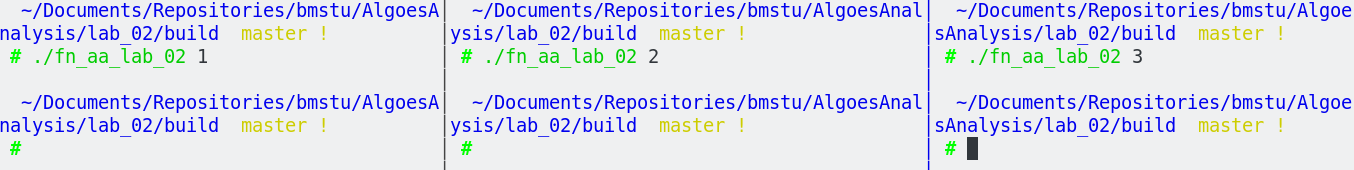
\includegraphics[scale=0.45]{images/test1.png}
    \caption{Пустой ввод}
    \label{img:zero-arg}
\end{figure}

\begin{figure}[H]
    \centering
    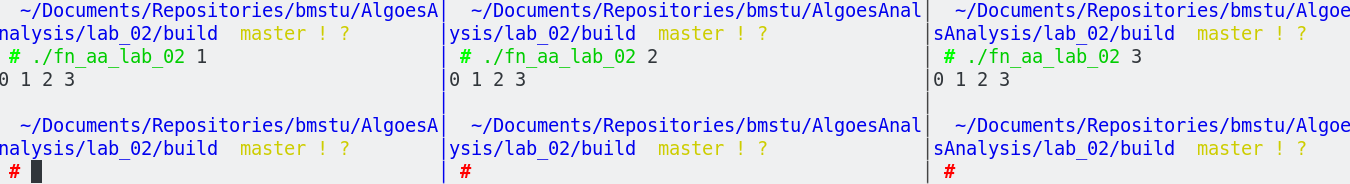
\includegraphics[scale=0.45]{images/test2.png}
    \caption{Невозможный размер}
    \label{img:zero-arg}
\end{figure}

\begin{figure}[H]
    \centering
    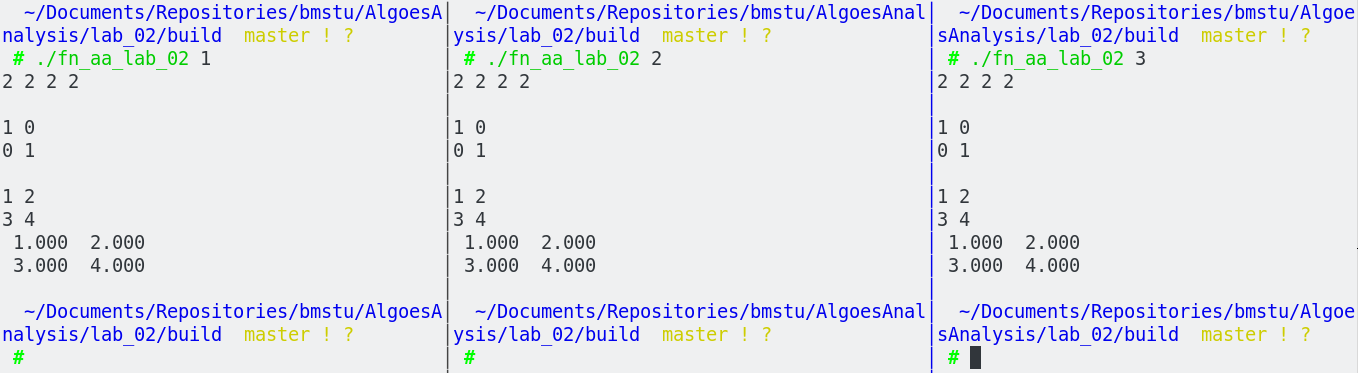
\includegraphics[scale=0.45]{images/test3.png}
    \caption{Корректный ввод}
    \label{img:zero-arg}
\end{figure}


\section{Описание тестирования}

Для проверки корректной работы реализованной программы были подготовлены тестовые данные, представленные в таблице 3.1.
\begin{table}[H]
    \caption{Тестовые данные и ожидаемые результаты}
    \centering
    \begin{tabular}{|c|c|c|}
        \hline
        Первая матрица & Вторая матрица & Ожидаемый результат \\
        \hline
        1 2 & 1 2 & \ 7 10 \\
        3 4 & 3 4 & 15 22 \\
        \hline
        1 2 3 & 1 2 3 & \ 30\ \ 36\ \ 42 \\
        4 5 6 & 4 5 6 & \ 66\ \ 81\ \ 96 \\
        7 8 9 & 7 8 9 & 102 126 150 \\
        \hline
        1 2 3 & 1 & 14 \\
        4 5 6 & 2 & 32 \\
              & 3 & \\
        \hline
    \end{tabular}
\end{table}

Тестирование было проведено успешно. Его результаты приведены в таблицах 3.2, 3.3, 3.4.
\begin{table}[H]
    \caption{Результаты тестирования стандартного алгоритма}
    \centering
    \begin{tabular}{|c|c|c|}
        \hline
        Первая матрица & Вторая матрица & Полученный результат \\
        \hline
        1 2 & 1 2 & \ 7 10 \\
        3 4 & 3 4 & 15 22 \\
        \hline
        1 2 3 & 1 2 3 & \ 30\ \ 36\ \ 42 \\
        4 5 6 & 4 5 6 & \ 66\ \ 81\ \ 96 \\
        7 8 9 & 7 8 9 & 102 126 150 \\
        \hline
        1 2 3 & 1 & 14 \\
        4 5 6 & 2 & 32 \\
              & 3 & \\
        \hline
    \end{tabular}
\end{table}
\begin{table}[H]
    \caption{Результаты тестирования алгоритма Винограда}
    \centering
    \begin{tabular}{|c|c|c|}
        \hline
        Первая матрица & Вторая матрица & Полученный результат \\
        \hline
        1 2 & 1 2 & \ 7 10 \\
        3 4 & 3 4 & 15 22 \\
        \hline
        1 2 3 & 1 2 3 & \ 30\ \ 36\ \ 42 \\
        4 5 6 & 4 5 6 & \ 66\ \ 81\ \ 96 \\
        7 8 9 & 7 8 9 & 102 126 150 \\
        \hline
        1 2 3 & 1 & 14 \\
        4 5 6 & 2 & 32 \\
              & 3 & \\
        \hline
    \end{tabular}
\end{table}
\begin{table}[H]
    \caption{Результаты тестирования модифицированного алгоритма Винограда}
    \centering
    \begin{tabular}{|c|c|c|}
        \hline
        Первая матрица & Вторая матрица & Полученный результат \\
        \hline
        1 2 & 1 2 & \ 7 10 \\
        3 4 & 3 4 & 15 22 \\
        \hline
        1 2 3 & 1 2 3 & \ 30\ \ 36\ \ 42 \\
        4 5 6 & 4 5 6 & \ 66\ \ 81\ \ 96 \\
        7 8 9 & 7 8 9 & 102 126 150 \\
        \hline
        1 2 3 & 1 & 14 \\
        4 5 6 & 2 & 32 \\
              & 3 & \\
        \hline
    \end{tabular}
\end{table}


\section{Вывод}
Для реализации программы были выбраны средства разработки: язык программирование C++, библиотека std::chrono, а так же подготовлены тестовые данные и успешно проведено тестирование.

